%%%%%%%%%%%%%%%%%%%%%%%%%%%%%%%%%%%%%%%%%%%%%%%%%%%%%%%%%%%%%%%%%%%%%%%%%%%%%%%%
%2345678901234567890123456789012345678901234567890123456789012345678901234567890
%        1         2         3         4         5         6         7         8

\documentclass[letterpaper, 10 pt, conference]{ieeeconf}  % Comment this line out
                                                          % if you need a4paper
%\documentclass[a4paper, 10pt, conference]{ieeeconf}      % Use this line for a4
                                                          % paper

\IEEEoverridecommandlockouts                              % This command is only
                                                          % needed if you want to
                                                          % use the \thanks command
\overrideIEEEmargins
% See the \addtolength command later in the file to balance the column lengths
% on the last page of the document



% The following packages can be found on http:\\www.ctan.org
\usepackage{graphics} % for pdf, bitmapped graphics files
\usepackage{epsfig} % for postscript graphics files
%\usepackage{mathptmx} % assumes new font selection scheme installed
%\usepackage{times} % assumes new font selection scheme installed
%\usepackage{amsmath} % assumes amsmath package installed
%\usepackage{amssymb}  % assumes amsmath package installed
\usepackage{graphicx}
\usepackage{listings}
\usepackage{color}
\usepackage{hyperref}

\definecolor{dkgreen}{rgb}{0,0.6,0}
\definecolor{gray}{rgb}{0.5,0.5,0.5}
\definecolor{mauve}{rgb}{0.58,0,0.82}

\lstset{frame=tb,
  language=bash,
  aboveskip=3mm,
  belowskip=3mm,
  showstringspaces=false,
  columns=flexible,
  basicstyle={\small\ttfamily},
  numbers=none,
  numberstyle=\tiny\color{gray},
  keywordstyle=\color{blue},
  commentstyle=\color{dkgreen},
  stringstyle=\color{mauve},
  breaklines=true,
  breakatwhitespace=true,
  tabsize=3
}

\title{\LARGE \bf
ET4394 Wireshark assignment W11
}

%\author{ \parbox{3 in}{\centering Huibert Kwakernaak*
%         \thanks{*Use the $\backslash$thanks command to put information here}\\
%         Faculty of Electrical Engineering, Mathematics and Computer Science\\
%         University of Twente\\
%         7500 AE Enschede, The Netherlands\\
%         {\tt\small h.kwakernaak@autsubmit.com}}
%         \hspace*{ 0.5 in}
%         \parbox{3 in}{ \centering Pradeep Misra**
%         \thanks{**The footnote marks may be inserted manually}\\
%        Department of Electrical Engineering \\
%         Wright State University\\
%         Dayton, OH 45435, USA\\
%         {\tt\small pmisra@cs.wright.edu}}
%}

\author{Pradhayini Ramamurthy (4180437) and Hans Okkerman (4290453)% <-this % stops a space
}


\begin{document}



\maketitle
\thispagestyle{empty}
\pagestyle{empty}


%%%%%%%%%%%%%%%%%%%%%%%%%%%%%%%%%%%%%%%%%%%%%%%%%%%%%%%%%%%%%%%%%%%%%%%%%%%%%%%%
\begin{abstract}

This report details the procedure, results and analysis of the Wireshark assignment on security (W11) executed by group WN2. WiFi packets were sniffed using airodump-ng while traveling across parts of the country on a train and a bus. The captured data was analyzed for trends in security protocols, encryption and authentication methods. The most prevalent configuration was found to be the WPA2 security protocol implementing the CCMP encryption method and the PSK authentication method.

\end{abstract}


%%%%%%%%%%%%%%%%%%%%%%%%%%%%%%%%%%%%%%%%%%%%%%%%%%%%%%%%%%%%%%%%%%%%%%%%%%%%%%%%
\section{Introduction}
For the Wireless Networking course of Delft University of Technology an analysis had to be done on WiFi networks. This report covers assignment $W11$ which concerns extracting the used security types per access point. To extract the required information dedicated software such as Wireshark and airodump-ng are used on a laptop which is carried through several areas to record data from nearby networks. 

The rest of this report is built up as follows: First the used software, hardware and data collection process are discussed. Next, the results of filtering the recorded data are shown. Finally conclusions are drawn about the used security of the networks. 



\section{Data collection}
\subsection{Tools}
The hardware used during this assignment was a DELL XPS 13 laptop running $Ubuntu 16.04$ and containing an $Intel Wireless 8260$ adapter that conforms to the IEEE 802.11 standard. Data collection was initially performed using Wireshark and tshark, with the wireless interface configured to operate in the $monitoring$ mode. However, as the data captured with these tools did not provide much insight into the security aspects of the monitored WiFi Access Points (APs), it was decided to use airodump-ng from the aircrack-ng package. There were three main advantages to making this choice. First, with airodump-ng the WiFi interface could be configured to operate in the $monitoring$ mode with little to no extra effort, unlike Wireshark which required a separate script to enable this configuration. Second, airodump-ng allowed the capture of data from multiple channels by doing an automatic, timed, channel hopping. This was both easy to configure (simply by omitting the $channel$ parameter specification) and fruitful in terms of the gathered data. Finally, the data dump from a run of airodump-ng provided information on the basic security configurations of an AP, in addition to the details provided by Wireshark. 

\subsection{Environment}
The analysis done for this assignment for focused on capturing data from a wide and varied geographical area, represented by the train route between Breda and Eindhoven and a bus route inside the city of Eindhoven. Several trial runs were done on both routes and the final data analysis was performed on a set of captures executed during the peak travel hours on a weekday. A few obvious expectations were confirmed with respect to the data trends from a superficial glance at the type and quantity of the data gathered. For instance, the density of WiFi APs inside a densely populated urban area such as Eindhoven was much higher than the distribution over the long and sparsely populated train route. This resulted in the number of observed unique APs over the 20 minute bus ride being over twice as many as the number observed in the 40 minute train ride. In contrast, the number of devices (202 devices) that were probing for a recognized, available AP on the train route was nearly 4.4 times the number of devices (46 devices) doing the same on the bus route. This could clearly be attributed to the number of mobile devices within range at the time of measurement. 

\subsection{Data Format and Characteristics}
Data collection was done using airodump-ng, configured to scan all channels by default (by periodically hopping channels) in both the 2.4GHz and 5GHz bands. The output was in the csv file format, which was then analyzed. No capture-time filtering could be done with airodump-ng and data filtering was done partly scripted and partly done manually. The following bash script snippet indicates the airodump-np capture. Output CSV files can be found in the \href{https://github.com/HOkkerman/ET4394/tree/master/wireshark_airodump_captures/airodump}{group git repository}.
\begin{lstlisting}
// startSniffing.sh

# Disable Network Manager
nmcli networking off

# Dump wifi sniffing data from all channels in csv format
sudo airodump-ng -b abg -e --write $output --output-format csv $interface

\end{lstlisting}
 
The data of interest for the security analysis of the wireless networks are given in the columns of $privacy$, $cipher$ and $authentication$ in the captured data dump. $Privacy$ contains the security protocol used by the network. These can be open or not encrypted, WEP which is an older standard that is no longer considered secure, WPA which replaced WEP and WPA2 which replaces WPA and is currently the most secure. $Cipher$ contains the used encryption protocol of the network. These are either none for open networks, $WEP$, $TKIP$ or $CCMP$. $TKIP$ is used by the WPA protocol and has been considered deprecated since 2009. $CCMP$ is the default encryption scheme for $WPA2$ which replaces $TKIP$, however it is possible to provide $TKIP$ on $WPA2$ to support older devices. Finally $authentication$ contains the means of client authentication to the network. This can be either none for open networks, $PSK$ for regular networks where a password is required to connect and $MGT$ for corporate or other more secure networks. These require a so called $RADIUS$ server which a user has to log on to and provide more information before he can connect to the network.
 
\section{Results}
From the recorded data several distribution profiles can be made based on security protocols, encryption types and authentication types. These will be discussed in the following sections. The measurements are provided in Table \ref{tab:measurements}.

\subsection{Security protocols}
Data was first collected while driving by bus through Eindhoven. The distribution of detected network security protocols can be seen in Figure \ref{fig:busencdist}. From the Figure it is clear that most detected networks support $WPA2$ or both $WPA2$ and $WPA$ and very few only support $WPA$ or even $WEP$. A rather large amount of open networks was also detected. From the corresponding $ESSID$s it can be shown that a large amount of these networks belong to KPN's $Fon$ network which enables an unencrypted, open AP on the routers of KPN's customers (SSID $KPN Fon$) by default. This (from personal experience) is something that a majority of users are unaware of and keep enabled, as seen by the $41$ or so such APs. The remaining open networks are mostly "free WiFi" hotspots in stores or cafeterias. 

\begin{figure}[h]
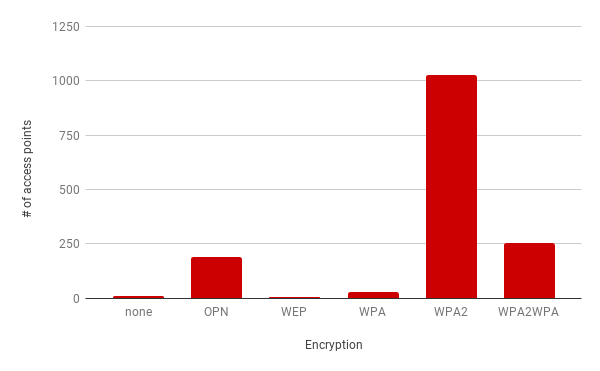
\includegraphics[scale=0.5]{Figures/BusEncryptionCount.png}
\caption{Security protocol distribution as measured on the bus}
\label{fig:busencdist}
\end{figure}

In Figure \ref{fig:trainencdist} the same data can be seen when traveling by train between Breda and Eindhoven. Roughly the same proportions as before can be observed except for an increase in the relative amount of open networks. Again a large amount of those networks are part of KPN's $Fon$ network or hotspots in stores, but now many "HotspotArriva" and "WiFi in de trein" are available as well. These last two are the open networks in the train as provided by Arriva and NS respectively.


\begin{figure}[h]
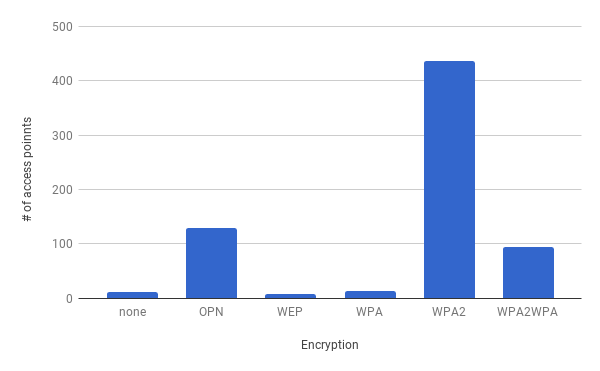
\includegraphics[scale=0.5]{Figures/TrainEncryptionCount.png}
\caption{Security protocol distribution as measured on the train}
\label{fig:trainencdist}
\end{figure}

Figure \ref{fig:encdist} shows the distributions from the bus and train measurements side by side. Here the larger proportion of open networks as measured in the train is clearly visible.

\begin{figure}[h]
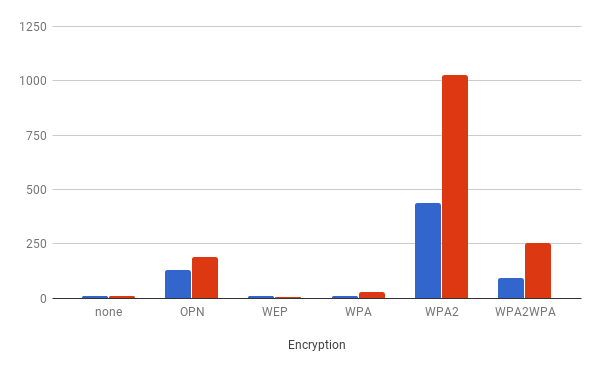
\includegraphics[scale=0.4]{Figures/EncryptionDist.png}
\caption{Security protocol distribution as measured on the train and bus}
\label{fig:encdist}
\end{figure}




\subsection{Encryption types}
When focusing on the most common $WPA$ and $WPA2$ protected networks another distribution can be made regarding the used encryption protocol. Figure \ref{fig:buscipher} shows that nearly all $WPA2$ networks as detected from the bus support the $CCMP$ encryption scheme with roughly one fifth supporting both $CCMP$ and the older $TKIP$. Of the networks supporting both $WPA$ and $WPA2$ most support both $CCMP$ and $TKIP$ with roughly one sixth only supporting $CCMP$. Networks that support $WPA2$ but only use $TKIP$ are nearly non-existent, which makes sense as it has been replaced by $CCMP$ and is only used to support old devices. Very few networks only supported $WPA$, which leads to a lack of usable statistics for these networks as seen in Figure \ref{fig:buscipher}. This is however a good sign as it means that not many networks are relying solely on older, deprecated security measures. 

Figure \ref{fig:traincipher} shows a similar distribution for the networks detected from the train ride, although it is not entirely clear what causes the difference in proportions between networks that support both $WPA$ and $WPA2$ and use $CCMP$ and $TKIP$, and those that only support $CCMP$. Again, not enough $WPA$-only networks were detected to make a proper comparison.



\begin{figure}[h]
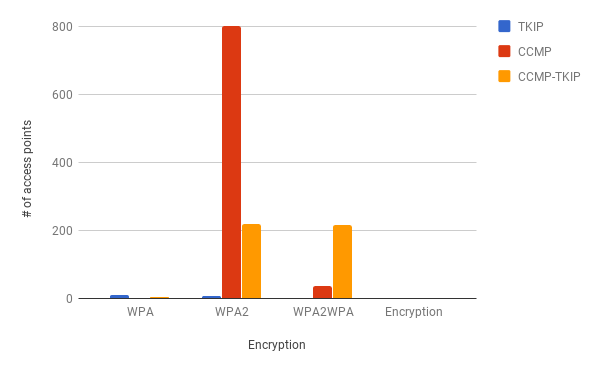
\includegraphics[scale=0.4]{Figures/CipherBus.png}
\caption{Encryption distribution as measured on bus}
\label{fig:buscipher}
\end{figure}


\begin{figure}[h]
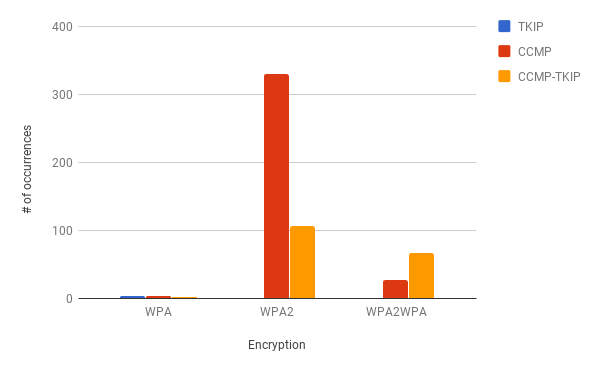
\includegraphics[scale=0.4]{Figures/CipherTrain.png}
\caption{Encryption distribution as measured on train}
\label{fig:traincipher}
\end{figure}




\subsection{Authentication types}
$WPA$ and $WPA2$ support two different client authentication methods, $PSK$ and $MGT$. As discussed before, $PSK$ or Pre-Shared Key, is the typical method of authentication used in home networks where users know the password of the network. $MGT$ uses a so called $RADIUS$ server that requires more information from the clients and is often used in corporate or other professional settings. Figures \ref{fig:busauth} and \ref{fig:trainauth} both show similar results for recordings from the bus and train respectively. It can be clearly seen that the large majority of networks support $PSK$. This makes sense as most home networks use this method. From the $ESSID$s it can be seen that most of the networks that support $MGT$ are called "ziggo". It is expected that this is a similar service as KPN's $Fon$ network, but ran by Ziggo. Another well known network that shows up in the records is "eduroam", which is a good example of the more advanced login requirements of $MGT$ authentication. Finally some companies seem to use the method as well.

\begin{figure}[h]
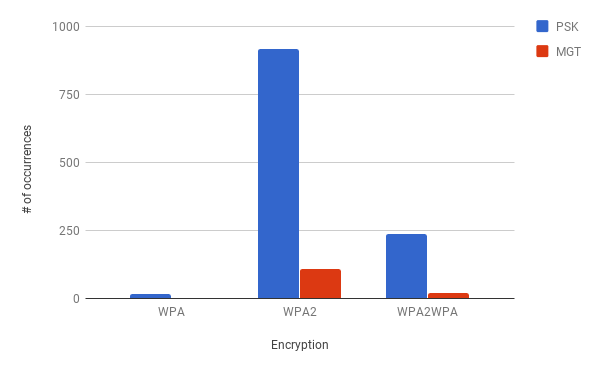
\includegraphics[scale=0.4]{Figures/AuthBus.png}
\caption{Authentication method distribution as measured on bus}
\label{fig:busauth}
\end{figure}


\begin{figure}[h]
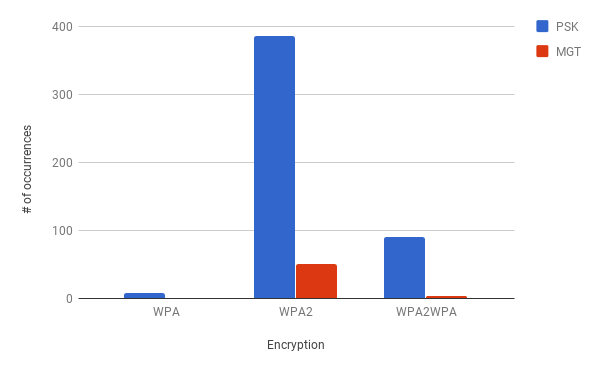
\includegraphics[scale=0.4]{Figures/AuthTrain.png}
\caption{Authentication method distribution as measured on train}
\label{fig:trainauth}
\end{figure}


\section{Conclusion}
From the graphs in the previous sections it can be seen that the trends in both populated urban areas and in the sparse rural areas are nearly identical, and only differ in the actual number of Access Points. Open unencrypted networks that do not require any user authentication are mostly provided by KPN's $Fon$ network, public transport companies such as NS with $Wifi in de trein$ and Arriva's $ArrivaHotspot$, city centers ($EHV FREE WIFI$) and shopping centers. Most other personal or office-owned APs are running $WPA2$ or both $WPA$ and $WPA2$, and most of those use either only $CCMP$ or both $CCMP$ and $TKIP$. Authentication is most commonly done using $PSK$ with some corporations using $MGT$. Very few networks still only rely on older insecure standards such as $WEP$ or $WPA$ only, which is a good sign for the overall security of wireless networks.

\begin{center}
  \begin{table*}
   \centering
    \begin{tabular}{ |l|l|l|l|l|l|l|l|l|l|l|l|l| }
    \hline    
    {} & \multicolumn{2}{|c|}{} & \multicolumn{6}{|c|}{Cipher} & \multicolumn{4}{|c|}{Authentication} \\ \hline
    {} & \multicolumn{2}{|c|}{Total} & \multicolumn{2}{|c|}{TKIP} & \multicolumn{2}{|c|}{CCMP} & \multicolumn{2}{|c|}{CCMP-TKIP} & \multicolumn{2}{|c|}{PSK} & \multicolumn{2}{|c|}{MGT} \\ \hline
    Security Protocol & Bus & Train& Bus & Train & Bus & Train & Bus & Train & Bus & Train & Bus & Train \\ \hline
    Unspecified & 12 & 12 & - & - & - & - & - & - & - & - & - & - \\ \hline
    OPN & 190 & 129 & - & - & - & - & - & - & - & - & - & - \\ \hline
    WEP & 5 & 9 & - & - & - & - & - & - & - & - & - & - \\ \hline    
    WPA & 29 & 13 & 10 & 3 & 1 & 3 & 4 & 2 & 15 & 8 & 0 & 0 \\ \hline
    WPA2 & 1024 & 436 & 6 & 0 & 800 & 330 & 218 & 106 & 916 & 385 & 108 & 51 \\ \hline
    WPA2WPA & 255 & 94 & 2 & 0 & 36 & 27 & 217 & 67 & 235 & 90 & 20 & 4 \\ \hline    
    \end{tabular}
    \caption{Distribution of number of occurrences of protocols in airodump-ng measurements}
    \label{tab:measurements}
  \end{table*}
\end{center}


\addtolength{\textheight}{-12cm}   % This command serves to balance the column lengths
                                  % on the last page of the document manually. It shortens
                                  % the textheight of the last page by a suitable amount.
                                  % This command does not take effect until the next page
                                  % so it should come on the page before the last. Make
                                  % sure that you do not shorten the textheight too much.

%%%%%%%%%%%%%%%%%%%%%%%%%%%%%%%%%%%%%%%%%%%%%%%%%%%%%%%%%%%%%%%%%%%%%%%%%%%%%%%%



%%%%%%%%%%%%%%%%%%%%%%%%%%%%%%%%%%%%%%%%%%%%%%%%%%%%%%%%%%%%%%%%%%%%%%%%%%%%%%%%



%%%%%%%%%%%%%%%%%%%%%%%%%%%%%%%%%%%%%%%%%%%%%%%%%%%%%%%%%%%%%%%%%%%%%%%%%%%%%%%% 





%\begin{thebibliography}{99}
%\bibitem{c1} G. O. Young, ÒSynthetic structure of industrial plastics (Book style with paper title and editor),Ó 	in Plastics, 2nd ed. vol. 3, J. Peters, Ed.  New York: McGraw-Hill, 1964, pp. 15Ð64.
%\end{thebibliography}




\end{document}
